\documentclass[tikz,border=5pt]{standalone}
\usetikzlibrary{arrows.meta}
\usetikzlibrary{backgrounds}
\usetikzlibrary{calc}

\usepackage{mathtools}
\newcommand*{\TickSize}{2pt}%

\begin{document}
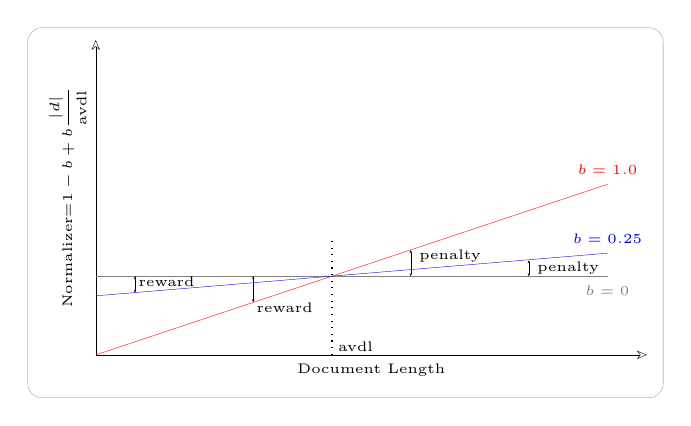
\begin{tikzpicture}
	[framed,background rectangle/.style={ultra thin, rounded corners=5pt, draw=gray}];

	%Axis
	\coordinate (x) at (7,0);
	\coordinate (y) at (0,4);
	\coordinate (o) at (0,0);
	\draw[-{Stealth[scale=1.0,angle'=45,open]}, line width=0.05mm] (o)--(x) node [midway, below, sloped, align=center]{\tiny Document Length};
	\draw[-{Stealth[scale=1.0,angle'=45,open]}, line width=0.05mm] (o)--(y) node [midway, above, sloped, align=center] {\tiny Normalizer=$1-b+b\dfrac{|d|}{\textrm{avdl}}$};
	\node at (3.3,0.1) {\tiny avdl};
	\draw[dotted] (3,0) --(3,1.5);

	\draw[gray,line width=0.05mm] plot [domain=0:6.5] (\x,{1}) node[anchor=north]{\tiny $b = 0$} ;
	\draw[blue,line width=0.05mm] plot [domain=0:6.5] (\x,{1-0.25+0.25*(\x/3)}) node[anchor=south]{\tiny $b = 0.25$} ;
	%\draw[red] plot [domain=0:6] (\x,{1-0.75+0.75*(\x/3)}) node[anchor=west]{\tiny $b = .75$} ;
	\draw[red,line width=0.05mm] plot [domain=0:6.5] (\x,{1-1+1*(\x/3)}) node[anchor=south]{\tiny $b = 1.0$} ;

	\draw[{Stealth[scale=0.3,angle'=45]}-{Stealth[scale=0.3,angle'=45]}, ultra thin] (4,1) -- (4,1.33);
	\node at (4.5,1.25) {\tiny penalty};
	\draw[{Stealth[scale=0.3,angle'=45]}-{Stealth[scale=0.3,angle'=45]}, ultra thin] (5.5,1) -- (5.5,1.2);
	\node at (6.0,1.1) {\tiny penalty};

	\draw[{Stealth[scale=0.3,angle'=45]}-{Stealth[scale=0.3,angle'=45]}, ultra thin] (2,1) -- (2,0.67);
	\node at (2.4,0.60) {\tiny reward};
	\draw[{Stealth[scale=0.3,angle'=45]}-{Stealth[scale=0.3,angle'=45]}, ultra thin] (0.5,1) -- (0.5,0.79);
	\node at (0.9,0.93) {\tiny reward};
\end{tikzpicture}
\end{document}